\documentclass[12pt,a4paper]{article}
\usepackage[utf8]{inputenc}
\usepackage[margin=1in]{geometry}
\usepackage{graphicx}
\usepackage{tikz}
\usepackage{xcolor}
\usepackage{hyperref}
\usepackage{listings}
\usepackage{float}
\usepackage{amsmath}
\usepackage{amssymb}
\usepackage{booktabs}
\usepackage{tcolorbox}
\usepackage{fancyhdr}

% TikZ libraries
\usetikzlibrary{shapes,shapes.geometric,arrows,positioning,shadows,decorations.pathmorphing,backgrounds,fit,calc,chains,matrix}
\usetikzlibrary{decorations.pathreplacing}

% Define colors
\definecolor{primaryblue}{RGB}{33,150,243}
\definecolor{secondarygreen}{RGB}{76,175,80}
\definecolor{accentorange}{RGB}{255,152,0}
\definecolor{darkgray}{RGB}{66,66,66}
\definecolor{lightgray}{RGB}{245,245,245}
\definecolor{codebg}{RGB}{40,44,52}

% Listings configuration
\lstset{
    language=Python,
    backgroundcolor=\color{codebg},
    basicstyle=\ttfamily\color{white}\small,
    keywordstyle=\color{orange},
    commentstyle=\color{green!60},
    stringstyle=\color{yellow!80},
    showstringspaces=false,
    breaklines=true,
    frame=single,
    rulecolor=\color{primaryblue},
    numbers=left,
    numberstyle=\tiny\color{gray},
}

% Page style
\pagestyle{fancy}
\fancyhf{}
\fancyhead[L]{\leftmark}
\fancyhead[R]{\thepage}
\fancyfoot[C]{SMARTqA - Autonomous QA Agent}

% Title information
\title{
    \vspace{-2cm}
    \begin{tikzpicture}[remember picture,overlay]
        \node[anchor=north,yshift=-3cm] at (current page.north) {
            \begin{tikzpicture}
                \fill[primaryblue!20] (0,0) rectangle (15,8);
                \node at (7.5,6) {\Huge\bfseries\color{primaryblue} SMARTqA};
                \node at (7.5,5) {\Large\color{darkgray} Autonomous QA Agent};
                \node[align=center] at (7.5,3.5) {\large\color{darkgray} 
                    Intelligent Test Case \& Selenium Script Generation\\
                    from Documentation};
                \node at (7.5,2) {\large\color{secondarygreen} \textbf{Technical Documentation}};
                \draw[primaryblue,line width=3pt] (1,1) -- (14,1);
            \end{tikzpicture}
        };
    \end{tikzpicture}
    \vspace{8cm}
}

\author{
    \textbf{Ayush Pandey}\\
    \texttt{@AyushPandey003}
}
\date{\today}

\begin{document}

\maketitle
\thispagestyle{empty}
\newpage

\tableofcontents
\newpage

% ============================================
\section{Executive Summary}
% ============================================

\begin{tcolorbox}[colback=primaryblue!5,colframe=primaryblue,title=Project Overview]
\textbf{SMARTqA} is an intelligent, autonomous QA agent that revolutionizes test automation by constructing a "testing brain" from project documentation. It leverages Retrieval-Augmented Generation (RAG) to generate comprehensive test cases and executable Selenium scripts with zero hallucinations.
\end{tcolorbox}

\subsection{Key Capabilities}

\begin{itemize}
    \item \textbf{Documentation-Grounded Testing}: Zero hallucination test plans based on actual project specs
    \item \textbf{Multi-Format Support}: Ingests PDF, Markdown, TXT, JSON, and HTML documents
    \item \textbf{Intelligent Code Generation}: Production-ready Selenium scripts with explicit waits and error handling
    \item \textbf{Semantic Search}: FAISS-powered vector database for context retrieval
    \item \textbf{User-Friendly Interface}: Streamlit-based dashboard with real-time feedback
\end{itemize}

% ============================================
\section{System Architecture}
% ============================================

\subsection{High-Level Architecture}

The SMARTqA system follows a layered architecture with four primary components:

\begin{figure}[H]
\centering
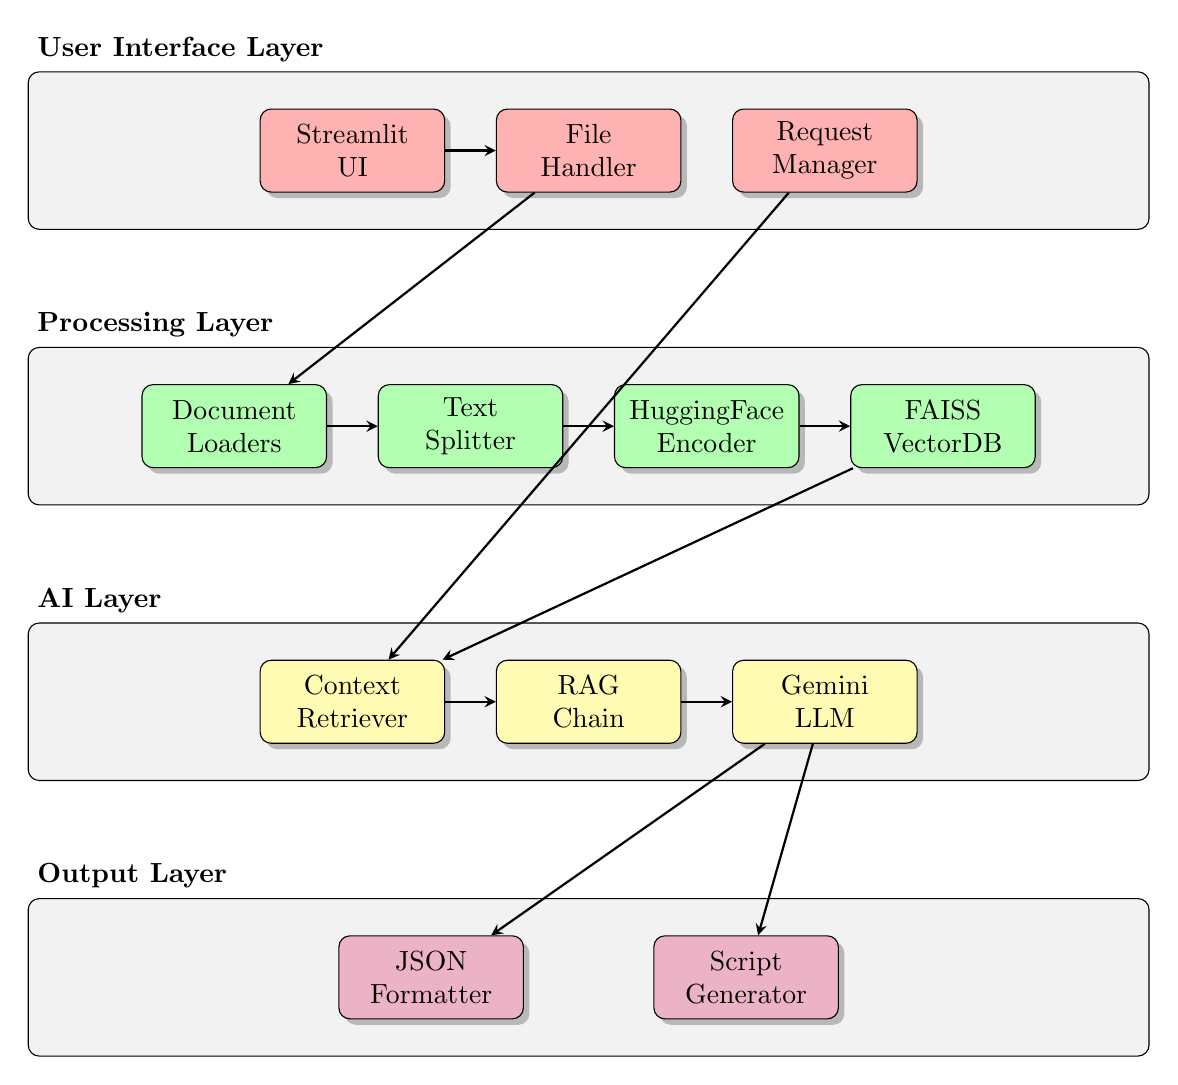
\begin{tikzpicture}[
    node distance=1.5cm,
    box/.style={rectangle, draw, fill=blue!20, text width=6em, text centered, rounded corners, minimum height=3em, drop shadow},
    layer/.style={rectangle, draw, fill=gray!10, text width=14cm, minimum height=2cm, rounded corners},
    arrow/.style={->, >=stealth, thick}
]

% Layers
\node[layer] (ui) at (0,0) {};
\node[above right] at (ui.north west) {\textbf{User Interface Layer}};

\node[layer] (proc) at (0,-3.5) {};
\node[above right] at (proc.north west) {\textbf{Processing Layer}};

\node[layer] (ai) at (0,-7) {};
\node[above right] at (ai.north west) {\textbf{AI Layer}};

\node[layer] (out) at (0,-10.5) {};
\node[above right] at (out.north west) {\textbf{Output Layer}};

% UI Layer components
\node[box, fill=red!30] (streamlit) at (-3,0) {Streamlit\\UI};
\node[box, fill=red!30] (filehandler) at (0,0) {File\\Handler};
\node[box, fill=red!30] (reqmgr) at (3,0) {Request\\Manager};

% Processing Layer components
\node[box, fill=green!30] (loader) at (-4.5,-3.5) {Document\\Loaders};
\node[box, fill=green!30] (splitter) at (-1.5,-3.5) {Text\\Splitter};
\node[box, fill=green!30] (encoder) at (1.5,-3.5) {HuggingFace\\Encoder};
\node[box, fill=green!30] (faiss) at (4.5,-3.5) {FAISS\\VectorDB};

% AI Layer components
\node[box, fill=yellow!30] (retriever) at (-3,-7) {Context\\Retriever};
\node[box, fill=yellow!30] (rag) at (0,-7) {RAG\\Chain};
\node[box, fill=yellow!30] (gemini) at (3,-7) {Gemini\\LLM};

% Output Layer components
\node[box, fill=purple!30] (json) at (-2,-10.5) {JSON\\Formatter};
\node[box, fill=purple!30] (script) at (2,-10.5) {Script\\Generator};

% Arrows
\draw[arrow] (streamlit) -- (filehandler);
\draw[arrow] (filehandler) -- (loader);
\draw[arrow] (loader) -- (splitter);
\draw[arrow] (splitter) -- (encoder);
\draw[arrow] (encoder) -- (faiss);
\draw[arrow] (reqmgr) -- (retriever);
\draw[arrow] (faiss) -- (retriever);
\draw[arrow] (retriever) -- (rag);
\draw[arrow] (rag) -- (gemini);
\draw[arrow] (gemini) -- (json);
\draw[arrow] (gemini) -- (script);

\end{tikzpicture}
\caption{SMARTqA Layered Architecture}
\end{figure}

% ============================================
\subsection{Component Interaction Diagram}
% ============================================

\begin{figure}[H]
\centering
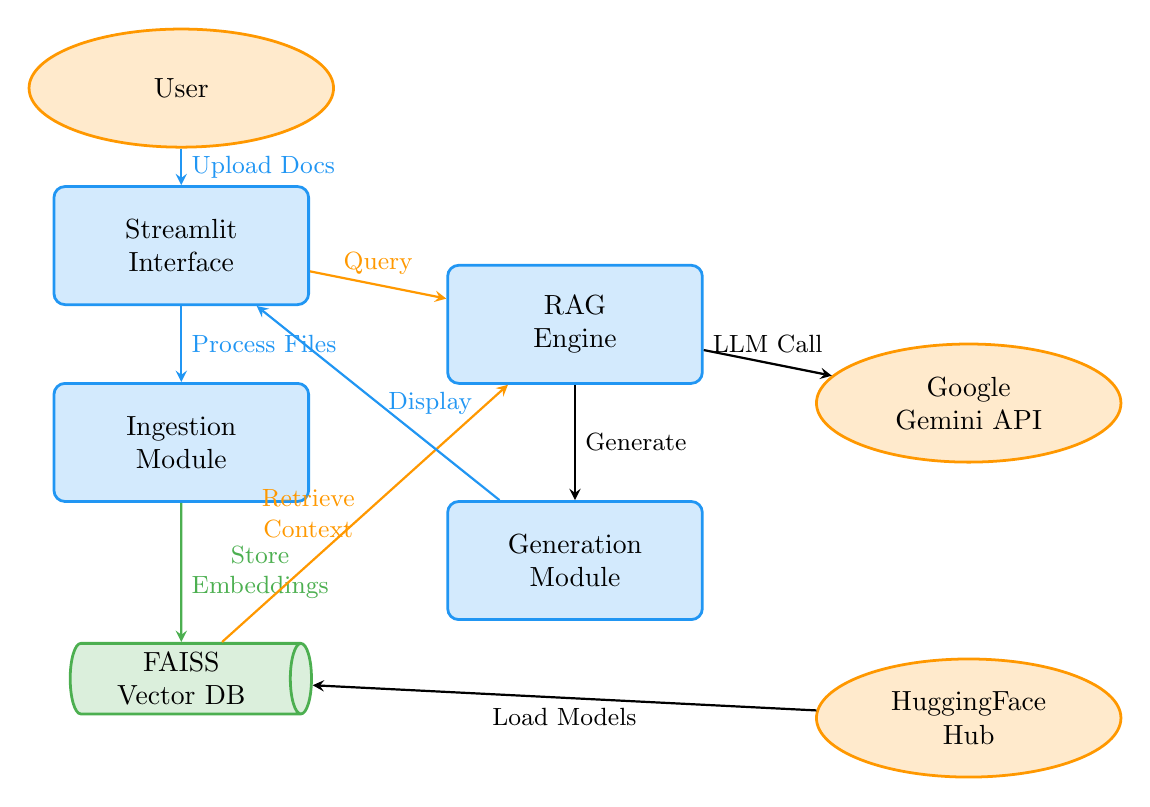
\begin{tikzpicture}[
    component/.style={rectangle, draw=primaryblue, line width=1pt, fill=primaryblue!20, text width=3cm, text centered, rounded corners, minimum height=1.5cm, align=center},
    storage/.style={cylinder, draw=secondarygreen, line width=1pt, fill=secondarygreen!20, text width=2.5cm, text centered, minimum height=2cm, aspect=0.3, cylinder uses custom fill, cylinder body fill=secondarygreen!20, cylinder end fill=secondarygreen!30, align=center},
    external/.style={ellipse, draw=accentorange, line width=1pt, fill=accentorange!20, text width=2.5cm, text centered, minimum height=1.5cm, align=center},
    arrow/.style={->, >=stealth, thick}
]

% External services
\node[external] (user) at (0,6) {User};
\node[external] (gemini) at (10,2) {Google\\Gemini API};
\node[external] (hf) at (10,-2) {HuggingFace\\Hub};

% Components
\node[component] (streamlit) at (0,4) {Streamlit\\Interface};
\node[component] (ingestion) at (0,1.5) {Ingestion\\Module};
\node[component] (rag) at (5,3) {RAG\\Engine};
\node[component] (generation) at (5,0) {Generation\\Module};

% Storage
\node[storage] (vectordb) at (0,-1.5) {FAISS\\Vector DB};

% Connections
\draw[arrow, primaryblue] (user) -- node[right, font=\small] {Upload Docs} (streamlit);
\draw[arrow, primaryblue] (streamlit) -- node[right, font=\small] {Process Files} (ingestion);
\draw[arrow, secondarygreen] (ingestion) -- node[right, font=\small, align=center] {Store\\Embeddings} (vectordb);
\draw[arrow, accentorange] (streamlit) -- node[above, font=\small] {Query} (rag);
\draw[arrow, accentorange] (vectordb) -- node[left, font=\small, align=center] {Retrieve\\Context} (rag);
\draw[arrow] (rag) -- node[above, font=\small] {LLM Call} (gemini);
\draw[arrow] (hf) -- node[below, font=\small] {Load Models} (vectordb);
\draw[arrow] (rag) -- node[right, font=\small] {Generate} (generation);
\draw[arrow, primaryblue] (generation) -- node[right, font=\small] {Display} (streamlit);

\end{tikzpicture}
\caption{Component Interaction Flow}
\end{figure}

% ============================================
\section{Data Flow Architecture}
% ============================================

\subsection{Document Ingestion Pipeline}

\begin{figure}[H]
\centering
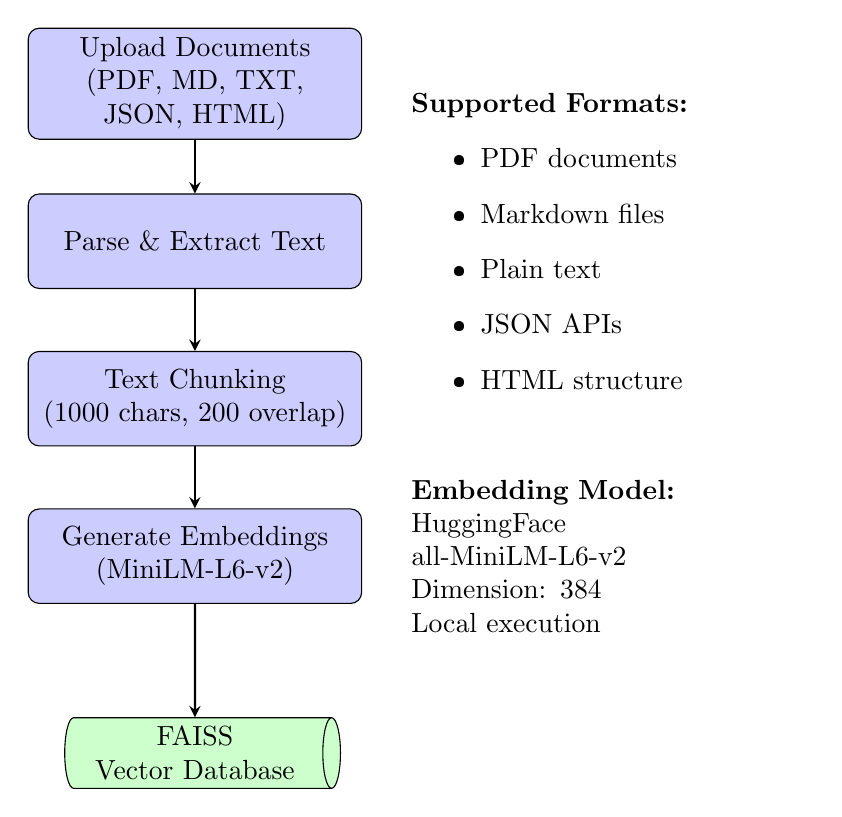
\begin{tikzpicture}[
    node distance=2cm,
    process/.style={rectangle, draw, fill=blue!20, text width=4cm, text centered, rounded corners, minimum height=1.2cm},
    decision/.style={diamond, draw, fill=yellow!20, text width=2.5cm, text centered, aspect=2},
    data/.style={cylinder, draw, fill=green!20, text width=3cm, text centered, minimum height=1.5cm, aspect=0.25},
    arrow/.style={->, >=stealth, thick}
]

\node[process] (upload) at (0,0) {Upload Documents\\(PDF, MD, TXT, JSON, HTML)};
\node[process] (parse) at (0,-2) {Parse \& Extract Text};
\node[process] (chunk) at (0,-4) {Text Chunking\\(1000 chars, 200 overlap)};
\node[process] (embed) at (0,-6) {Generate Embeddings\\(MiniLM-L6-v2)};
\node[data] (store) at (0,-8.5) {FAISS\\Vector Database};

\draw[arrow] (upload) -- (parse);
\draw[arrow] (parse) -- (chunk);
\draw[arrow] (chunk) -- (embed);
\draw[arrow] (embed) -- (store);

% Side annotations
\node[right=0.5cm of parse, text width=5cm, align=left] {
    \textbf{Supported Formats:}
    \begin{itemize}
        \item PDF documents
        \item Markdown files
        \item Plain text
        \item JSON APIs
        \item HTML structure
    \end{itemize}
};

\node[right=0.5cm of embed, text width=5cm, align=left] {
    \textbf{Embedding Model:}\\
    HuggingFace\\
    all-MiniLM-L6-v2\\
    Dimension: 384\\
    Local execution
};

\end{tikzpicture}
\caption{Document Ingestion Data Flow}
\end{figure}

% ============================================
\subsection{Test Case Generation Flow}
% ============================================

\begin{figure}[H]
\centering
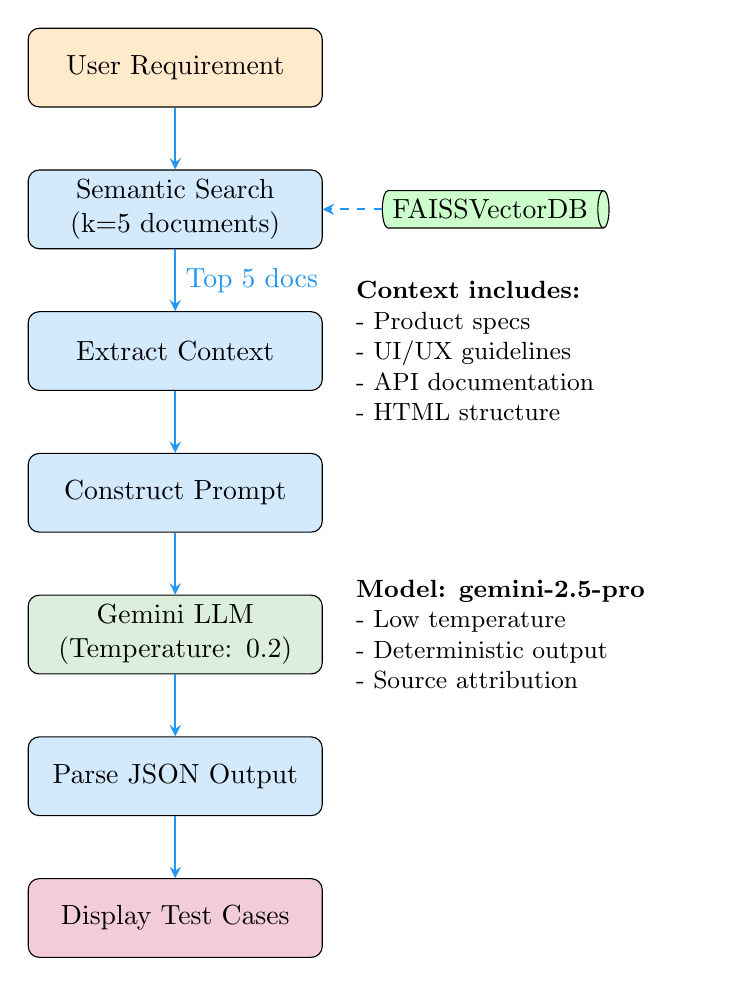
\begin{tikzpicture}[
    node distance=1.5cm,
    process/.style={rectangle, draw, fill=primaryblue!20, text width=3.5cm, text centered, rounded corners, minimum height=1cm},
    arrow/.style={->, >=stealth, thick, primaryblue}
]

\node[process, fill=accentorange!20] (req) at (0,0) {User Requirement};
\node[process] (semantic) at (0,-1.8) {Semantic Search\\(k=5 documents)};
\node[process] (context) at (0,-3.6) {Extract Context};
\node[process] (prompt) at (0,-5.4) {Construct Prompt};
\node[process, fill=secondarygreen!20] (llm) at (0,-7.2) {Gemini LLM\\(Temperature: 0.2)};
\node[process] (parse) at (0,-9) {Parse JSON Output};
\node[process, fill=purple!20] (display) at (0,-10.8) {Display Test Cases};

\draw[arrow] (req) -- (semantic);
\draw[arrow] (semantic) -- node[right] {Top 5 docs} (context);
\draw[arrow] (context) -- (prompt);
\draw[arrow] (prompt) -- (llm);
\draw[arrow] (llm) -- (parse);
\draw[arrow] (parse) -- (display);

% FAISS DB on the side
\node[cylinder, draw, fill=green!20, minimum height=2cm, aspect=0.3] (faiss) at (4,-1.8) {FAISS\\VectorDB};
\draw[arrow, dashed] (faiss) -- (semantic);

% Annotations
\node[right=0.3cm of context, text width=4.5cm, align=left, font=\small] {
    \textbf{Context includes:}\\
    - Product specs\\
    - UI/UX guidelines\\
    - API documentation\\
    - HTML structure
};

\node[right=0.3cm of llm, text width=4.5cm, align=left, font=\small] {
    \textbf{Model: gemini-2.5-pro}\\
    - Low temperature\\
    - Deterministic output\\
    - Source attribution
};

\end{tikzpicture}
\caption{Test Case Generation Process Flow}
\end{figure}

% ============================================
\section{Core Components}
% ============================================

\subsection{Module Breakdown}

\begin{table}[H]
\centering
\begin{tabular}{@{}lp{8cm}@{}}
\toprule
\textbf{Module} & \textbf{Responsibility} \\ \midrule
\texttt{app.py} & Main Streamlit interface, user interaction, workflow orchestration \\
\texttt{ingestion.py} & Document loading, text splitting, vector database creation \\
\texttt{rag.py} & LLM initialization and configuration \\
\texttt{generation.py} & Test case and Selenium script generation logic \\ \bottomrule
\end{tabular}
\caption{Core Module Responsibilities}
\end{table}

\subsection{Backend Module Architecture}

\begin{figure}[H]
\centering
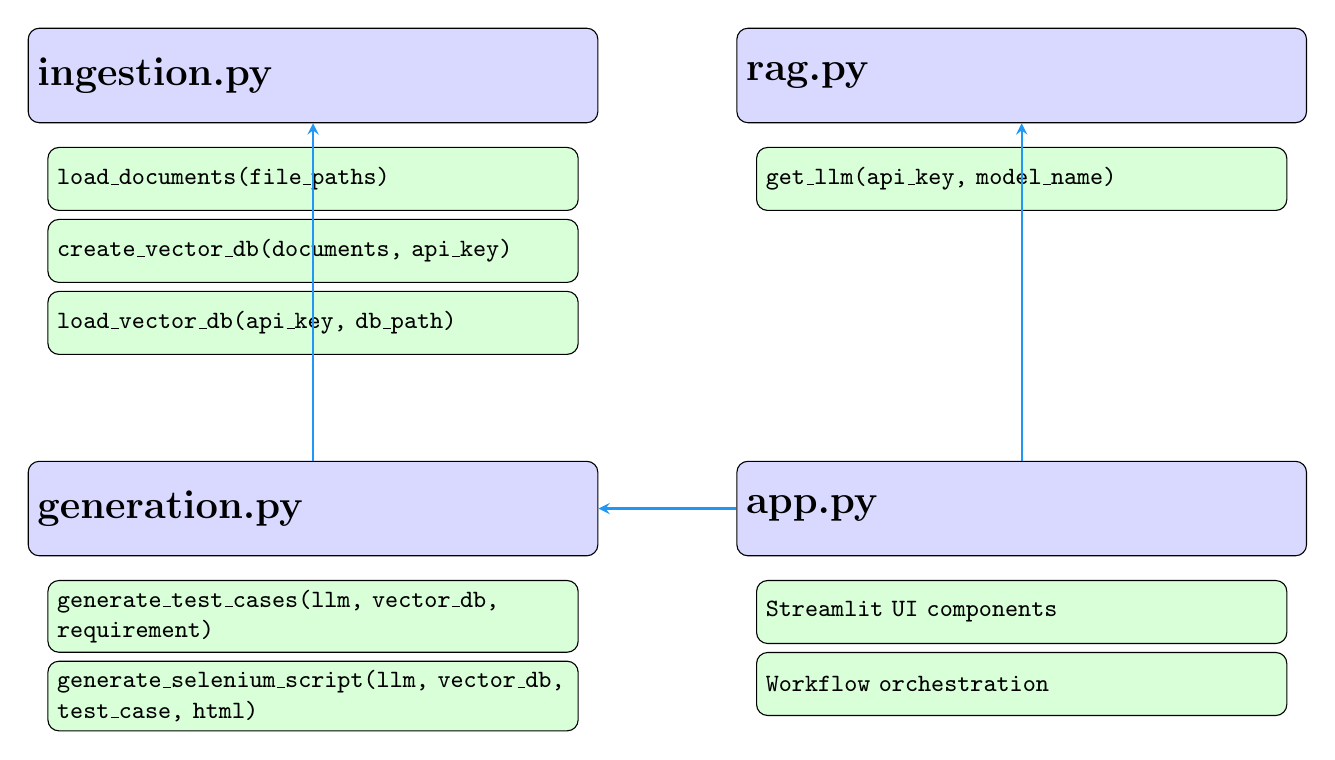
\begin{tikzpicture}[
    module/.style={rectangle, draw, fill=blue!15, text width=7cm, minimum height=1.2cm, rounded corners},
    function/.style={rectangle, draw, fill=green!15, text width=6.5cm, minimum height=0.8cm, rounded corners, font=\small}
]

% Modules
\node[module] (ingestion) at (0,0) {\Large\textbf{ingestion.py}};
\node[function, below=0.3cm of ingestion] (load) {\texttt{load\_documents(file\_paths)}};
\node[function, below=0.1cm of load] (create) {\texttt{create\_vector\_db(documents, api\_key)}};
\node[function, below=0.1cm of create] (loaddb) {\texttt{load\_vector\_db(api\_key, db\_path)}};

\node[module] (rag) at (9,0) {\Large\textbf{rag.py}};
\node[function, below=0.3cm of rag] (getllm) {\texttt{get\_llm(api\_key, model\_name)}};

\node[module] (generation) at (0,-5.5) {\Large\textbf{generation.py}};
\node[function, below=0.3cm of generation] (gentests) {\texttt{generate\_test\_cases(llm, vector\_db, requirement)}};
\node[function, below=0.1cm of gentests] (genselenium) {\texttt{generate\_selenium\_script(llm, vector\_db, test\_case, html)}};

\node[module] (app) at (9,-5.5) {\Large\textbf{app.py}};
\node[function, below=0.3cm of app] (streamlit) {\texttt{Streamlit UI components}};
\node[function, below=0.1cm of streamlit] (workflow) {\texttt{Workflow orchestration}};

% Connections
\draw[->, >=stealth, thick, primaryblue] (app.west) -- (generation.east);
\draw[->, >=stealth, thick, primaryblue] (app.north) -- (rag.south);
\draw[->, >=stealth, thick, primaryblue] (generation.north) -- (ingestion.south);

\end{tikzpicture}
\caption{Backend Module Structure}
\end{figure}

% ============================================
\section{Detailed Sequence Diagrams}
% ============================================

\subsection{Complete User Workflow}

\begin{figure}[H]
\centering
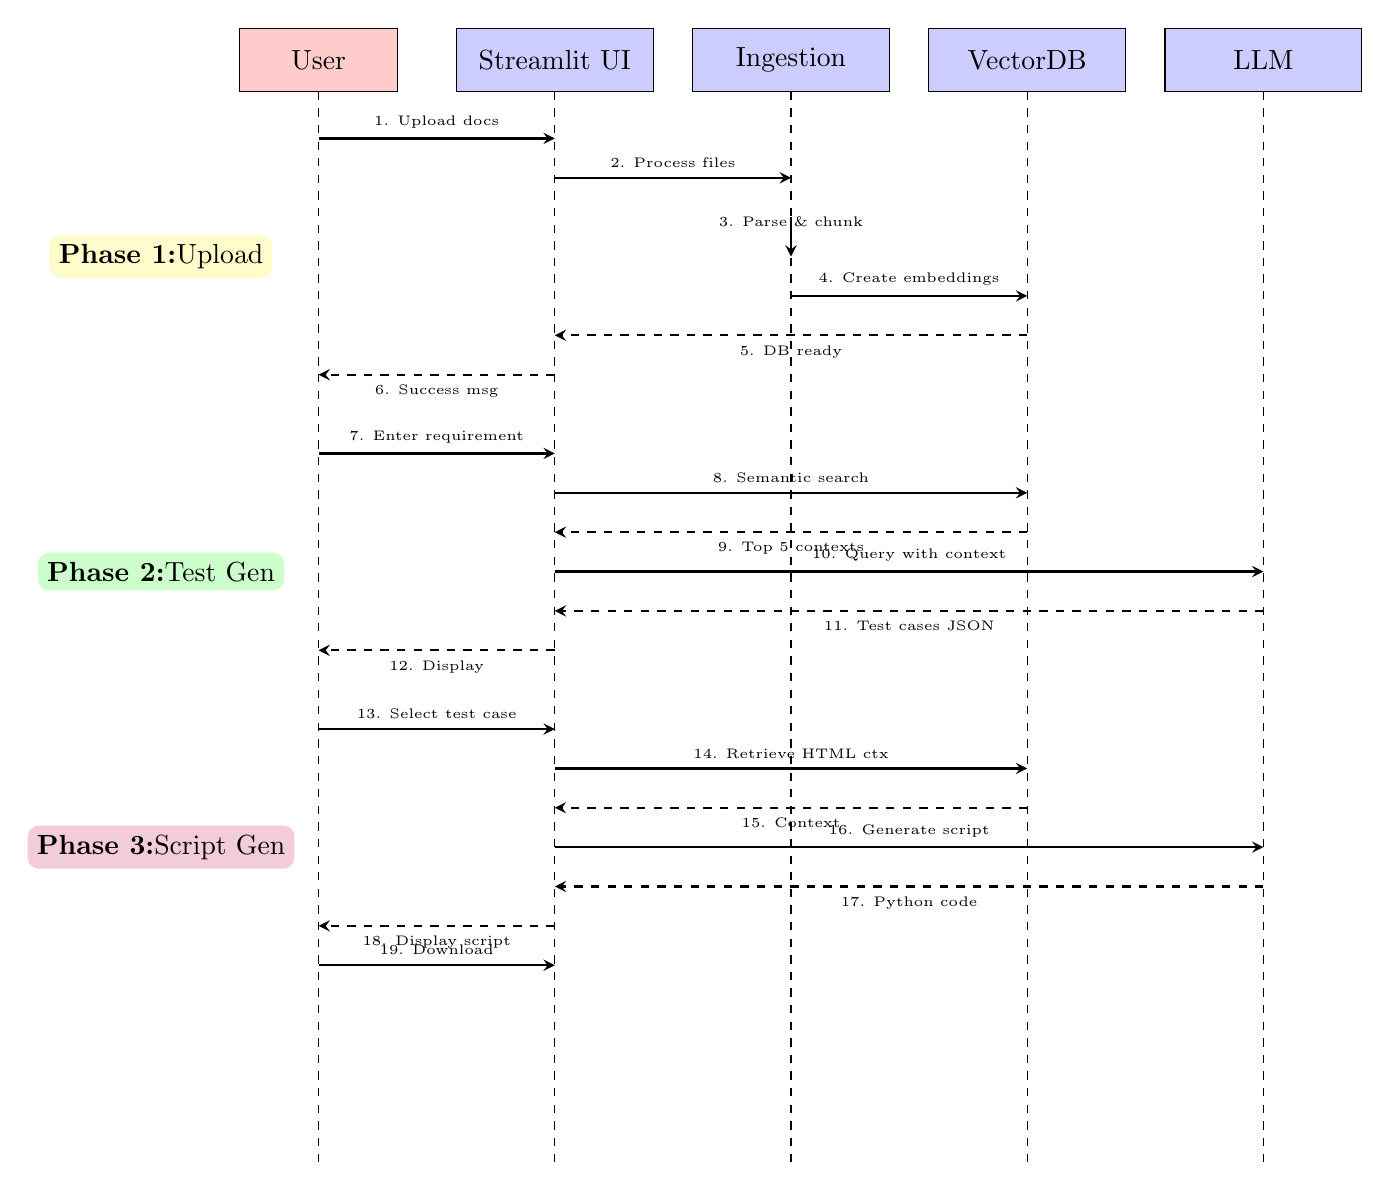
\begin{tikzpicture}[
    >=stealth,
    actor/.style={rectangle, draw, fill=red!20, minimum width=2cm, minimum height=0.8cm},
    participant/.style={rectangle, draw, fill=blue!20, minimum width=2.5cm, minimum height=0.8cm},
    message/.style={->, thick},
    return/.style={->, dashed, thick}
]

% Actors and Participants
\node[actor] (user) at (0,0) {User};
\node[participant] (ui) at (3,0) {Streamlit UI};
\node[participant] (ingest) at (6,0) {Ingestion};
\node[participant] (vdb) at (9,0) {VectorDB};
\node[participant] (llm) at (12,0) {LLM};

% Lifelines
\draw[dashed] (user) -- (0,-14);
\draw[dashed] (ui) -- (3,-14);
\draw[dashed] (ingest) -- (6,-14);
\draw[dashed] (vdb) -- (9,-14);
\draw[dashed] (llm) -- (12,-14);

% Messages - Document Upload Phase
\draw[message] (0,-1) -- node[above, font=\tiny] {1. Upload docs} (3,-1);
\draw[message] (3,-1.5) -- node[above, font=\tiny] {2. Process files} (6,-1.5);
\draw[message] (6,-2) -- node[above, font=\tiny] {3. Parse \& chunk} (6,-2.5);
\draw[message] (6,-3) -- node[above, font=\tiny] {4. Create embeddings} (9,-3);
\draw[return] (9,-3.5) -- node[below, font=\tiny] {5. DB ready} (3,-3.5);
\draw[return] (3,-4) -- node[below, font=\tiny] {6. Success msg} (0,-4);

% Messages - Test Generation Phase
\draw[message] (0,-5) -- node[above, font=\tiny] {7. Enter requirement} (3,-5);
\draw[message] (3,-5.5) -- node[above, font=\tiny] {8. Semantic search} (9,-5.5);
\draw[return] (9,-6) -- node[below, font=\tiny] {9. Top 5 contexts} (3,-6);
\draw[message] (3,-6.5) -- node[above, font=\tiny] {10. Query with context} (12,-6.5);
\draw[return] (12,-7) -- node[below, font=\tiny] {11. Test cases JSON} (3,-7);
\draw[return] (3,-7.5) -- node[below, font=\tiny] {12. Display} (0,-7.5);

% Messages - Script Generation Phase
\draw[message] (0,-8.5) -- node[above, font=\tiny] {13. Select test case} (3,-8.5);
\draw[message] (3,-9) -- node[above, font=\tiny] {14. Retrieve HTML ctx} (9,-9);
\draw[return] (9,-9.5) -- node[below, font=\tiny] {15. Context} (3,-9.5);
\draw[message] (3,-10) -- node[above, font=\tiny] {16. Generate script} (12,-10);
\draw[return] (12,-10.5) -- node[below, font=\tiny] {17. Python code} (3,-10.5);
\draw[return] (3,-11) -- node[below, font=\tiny] {18. Display script} (0,-11);
\draw[message] (0,-11.5) -- node[above, font=\tiny] {19. Download} (3,-11.5);

% Phase labels
\node[fill=yellow!20, rounded corners] at (-2,-2.5) {\textbf{Phase 1:}\\Upload};
\node[fill=green!20, rounded corners] at (-2,-6.5) {\textbf{Phase 2:}\\Test Gen};
\node[fill=purple!20, rounded corners] at (-2,-10) {\textbf{Phase 3:}\\Script Gen};

\end{tikzpicture}
\caption{Complete User Workflow Sequence}
\end{figure}

% ============================================
\section{Technology Stack}
% ============================================

\subsection{Technology Components}

\begin{figure}[H]
\centering
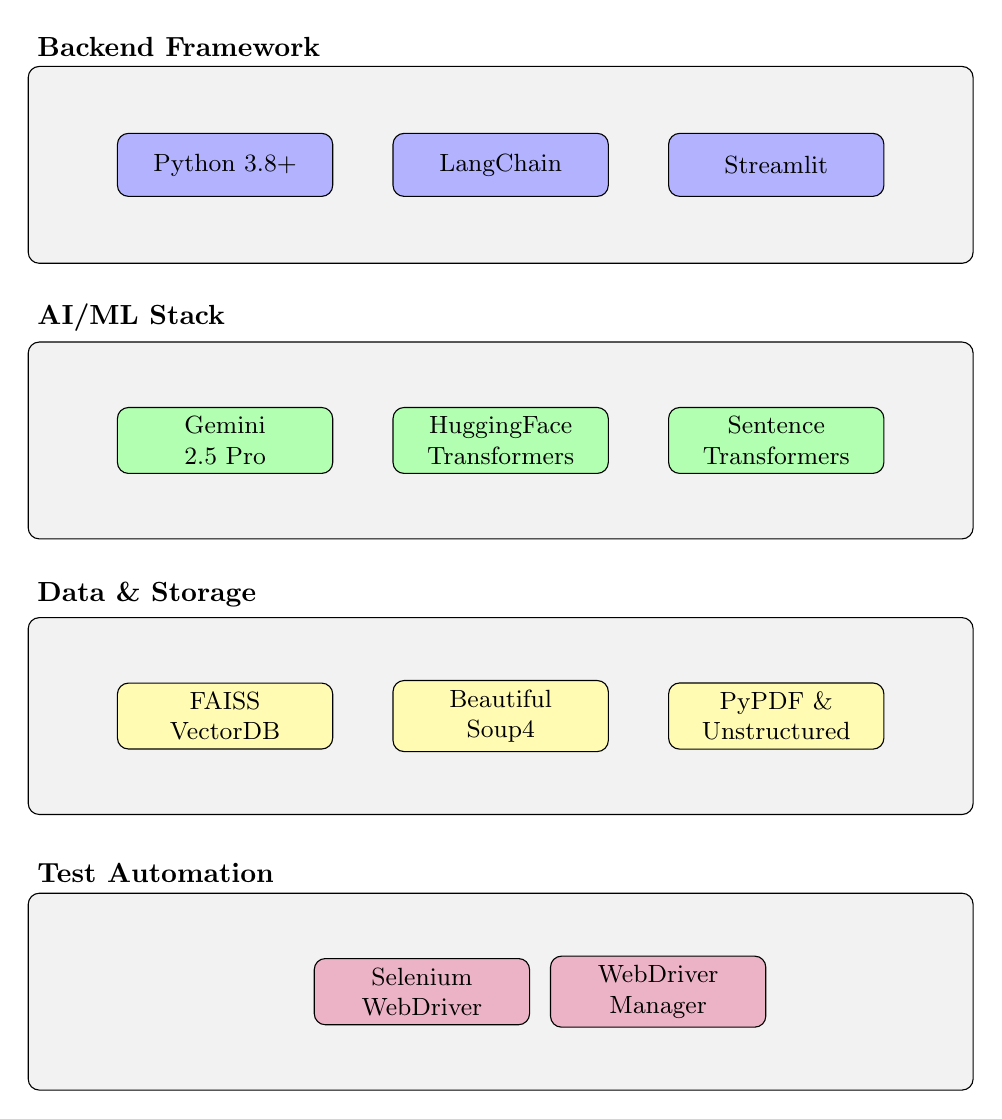
\begin{tikzpicture}[
    layer/.style={rectangle, draw, fill=gray!10, minimum width=12cm, minimum height=2.5cm, rounded corners},
    tech/.style={rectangle, draw, fill=blue!20, text width=2.5cm, text centered, rounded corners, minimum height=0.8cm, font=\small}
]

% Backend Layer
\node[layer] (backend) at (0,0) {};
\node[above right] at (backend.north west) {\textbf{Backend Framework}};
\node[tech, fill=blue!30] (python) at (-3.5,0) {Python 3.8+};
\node[tech, fill=blue!30] (langchain) at (0,0) {LangChain};
\node[tech, fill=blue!30] (streamlit) at (3.5,0) {Streamlit};

% AI/ML Layer
\node[layer] (ai) at (0,-3.5) {};
\node[above right] at (ai.north west) {\textbf{AI/ML Stack}};
\node[tech, fill=green!30] (gemini) at (-3.5,-3.5) {Gemini\\2.5 Pro};
\node[tech, fill=green!30] (hf) at (0,-3.5) {HuggingFace\\Transformers};
\node[tech, fill=green!30] (sent) at (3.5,-3.5) {Sentence\\Transformers};

% Data Layer
\node[layer] (data) at (0,-7) {};
\node[above right] at (data.north west) {\textbf{Data \& Storage}};
\node[tech, fill=yellow!30] (faiss) at (-3.5,-7) {FAISS\\VectorDB};
\node[tech, fill=yellow!30] (bs4) at (0,-7) {Beautiful\\Soup4};
\node[tech, fill=yellow!30] (pypdf) at (3.5,-7) {PyPDF \&\\Unstructured};

% Automation Layer
\node[layer] (auto) at (0,-10.5) {};
\node[above right] at (auto.north west) {\textbf{Test Automation}};
\node[tech, fill=purple!30] (selenium) at (-1,-10.5) {Selenium\\WebDriver};
\node[tech, fill=purple!30] (webdriver) at (2,-10.5) {WebDriver\\Manager};

\end{tikzpicture}
\caption{Technology Stack Layers}
\end{figure}

% ============================================
\section{Core Algorithms}
% ============================================

\subsection{RAG Pipeline Algorithm}

\begin{tcolorbox}[colback=lightgray,colframe=primaryblue,title=RAG Algorithm]
\begin{lstlisting}[language=Python]
def generate_test_cases(llm, vector_db, requirement):
    # Step 1: Initialize retriever
    retriever = vector_db.as_retriever(
        search_kwargs={"k": 5}
    )
    
    # Step 2: Define prompt template
    template = """You are an expert QA engineer...
    Context: {context}
    Requirement: {requirement}
    Output Format: JSON list of test cases..."""
    
    prompt = PromptTemplate.from_template(template)
    
    # Step 3: Build RAG chain
    rag_chain = (
        {
            "context": retriever | format_docs,
            "requirement": RunnablePassthrough()
        }
        | prompt | llm | StrOutputParser()
    )
    
    # Step 4: Execute and return
    return rag_chain.invoke(requirement)
\end{lstlisting}
\end{tcolorbox}

\subsection{Vector Embedding Process}

\begin{figure}[H]
\centering
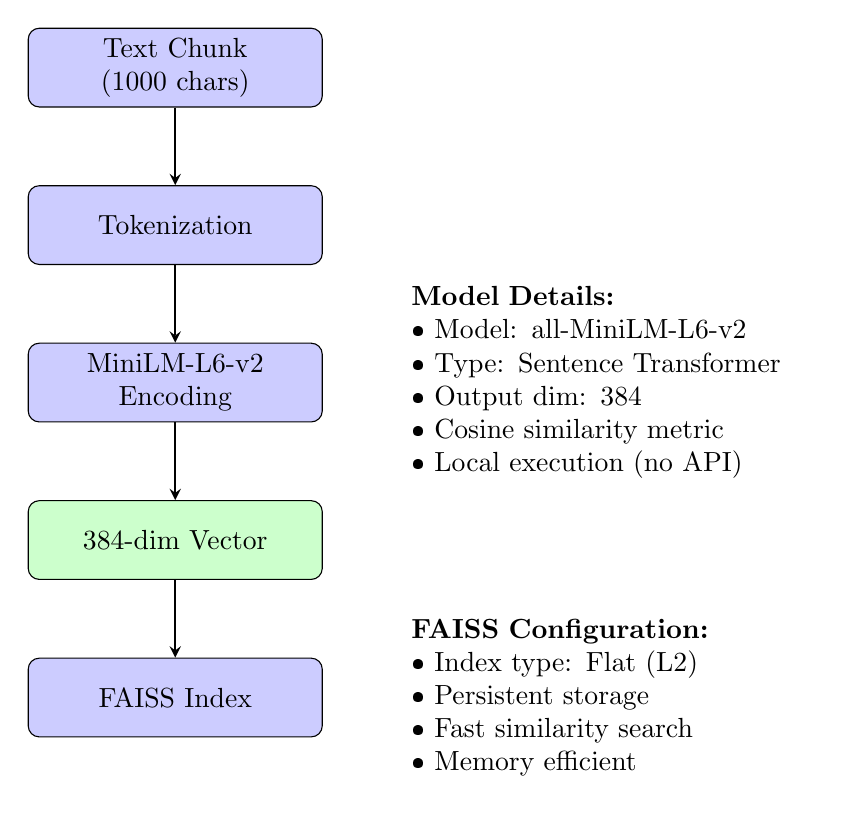
\begin{tikzpicture}[
    node distance=2cm,
    process/.style={rectangle, draw, fill=blue!20, text width=3.5cm, text centered, rounded corners, minimum height=1cm},
    arrow/.style={->, >=stealth, thick}
]

\node[process] (input) at (0,0) {Text Chunk\\(1000 chars)};
\node[process] (tokenize) at (0,-2) {Tokenization};
\node[process] (encode) at (0,-4) {MiniLM-L6-v2\\Encoding};
\node[process, fill=green!20] (vector) at (0,-6) {384-dim Vector};
\node[process] (index) at (0,-8) {FAISS Index};

\draw[arrow] (input) -- (tokenize);
\draw[arrow] (tokenize) -- (encode);
\draw[arrow] (encode) -- (vector);
\draw[arrow] (vector) -- (index);

% Side information
\node[right=1cm of encode, text width=5cm, align=left] {
    \textbf{Model Details:}\\
    • Model: all-MiniLM-L6-v2\\
    • Type: Sentence Transformer\\
    • Output dim: 384\\
    • Cosine similarity metric\\
    • Local execution (no API)
};

\node[right=1cm of index, text width=5cm, align=left] {
    \textbf{FAISS Configuration:}\\
    • Index type: Flat (L2)\\
    • Persistent storage\\
    • Fast similarity search\\
    • Memory efficient
};

\end{tikzpicture}
\caption{Vector Embedding Pipeline}
\end{figure}

% ============================================
\section{User Interface Design}
% ============================================

\subsection{Streamlit UI Structure}

\begin{figure}[H]
\centering
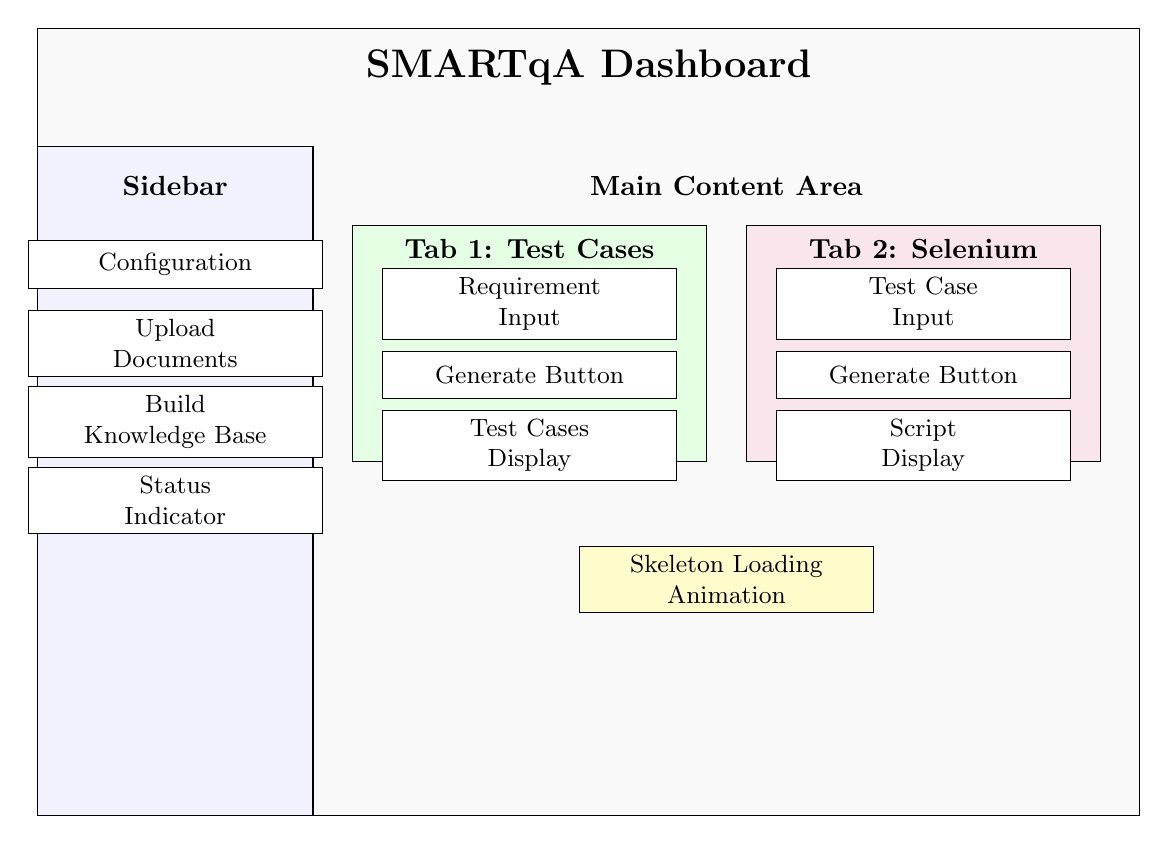
\begin{tikzpicture}[
    panel/.style={rectangle, draw, fill=blue!10, minimum width=4cm, minimum height=2cm, rounded corners},
    element/.style={rectangle, draw, fill=white, text width=3.5cm, text centered, minimum height=0.6cm, font=\small}
]

% Main layout
\draw[fill=gray!5] (0,0) rectangle (14,10);
\node at (7,9.5) {\Large\textbf{SMARTqA Dashboard}};

% Sidebar
\draw[fill=blue!5] (0,0) rectangle (3.5,8.5);
\node at (1.75,8) {\textbf{Sidebar}};
\node[element] (config) at (1.75,7) {Configuration};
\node[element] (upload) at (1.75,6) {Upload\\Documents};
\node[element] (build) at (1.75,5) {Build\\Knowledge Base};
\node[element] (status) at (1.75,4) {Status\\Indicator};

% Main content area
\node at (8.75,8) {\textbf{Main Content Area}};

% Tab 1
\draw[fill=green!10] (4,4.5) rectangle (8.5,7.5);
\node at (6.25,7.2) {\textbf{Tab 1: Test Cases}};
\node[element] (input1) at (6.25,6.5) {Requirement\\Input};
\node[element] (gen1) at (6.25,5.6) {Generate Button};
\node[element] (output1) at (6.25,4.7) {Test Cases\\Display};

% Tab 2
\draw[fill=purple!10] (9,4.5) rectangle (13.5,7.5);
\node at (11.25,7.2) {\textbf{Tab 2: Selenium}};
\node[element] (input2) at (11.25,6.5) {Test Case\\Input};
\node[element] (gen2) at (11.25,5.6) {Generate Button};
\node[element] (output2) at (11.25,4.7) {Script\\Display};

% Progress indicators
\node[element, fill=yellow!20] (progress) at (8.75,3) {Skeleton Loading\\Animation};

\end{tikzpicture}
\caption{Streamlit UI Layout}
\end{figure}

% ============================================
\section{Key Metrics and Performance}
% ============================================

\begin{table}[H]
\centering
\begin{tabular}{@{}lc@{}}
\toprule
\textbf{Metric} & \textbf{Value} \\ \midrule
Supported Document Formats & 5 (PDF, MD, TXT, JSON, HTML) \\
Embedding Dimension & 384 (MiniLM-L6-v2) \\
Context Window per Query & 5 documents \\
Text Chunk Size & 1000 characters \\
Chunk Overlap & 200 characters \\
LLM Temperature & 0.2 (deterministic) \\
Retrieval Strategy & Semantic similarity (FAISS) \\
Average Query Time & < 5 seconds \\
Embedding Model Size & ~80 MB (local) \\ \bottomrule
\end{tabular}
\caption{System Performance Metrics}
\end{table}

% ============================================
\section{Example Usage}
% ============================================

\subsection{Test Case Generation Example}

\begin{tcolorbox}[colback=lightgray,colframe=secondarygreen,title=Example Input]
\textbf{User Requirement:}\\
``Test the discount code functionality with valid and invalid codes''
\end{tcolorbox}

\begin{tcolorbox}[colback=lightgray,colframe=primaryblue,title=Generated Output]
\begin{verbatim}
[
  {
    "Test_ID": "TC_001",
    "Feature": "Discount Code Validation",
    "Test_Scenario": "Apply valid 20% discount code",
    "Expected_Result": "Discount applied, price reduced",
    "Grounded_In": "product_specs.md"
  },
  {
    "Test_ID": "TC_002",
    "Feature": "Discount Code Validation",
    "Test_Scenario": "Apply invalid discount code",
    "Expected_Result": "Error message displayed",
    "Grounded_In": "ui_ux_guide.txt"
  }
]
\end{verbatim}
\end{tcolorbox}

% ============================================
\section{Project Structure}
% ============================================

\begin{figure}[H]
\centering
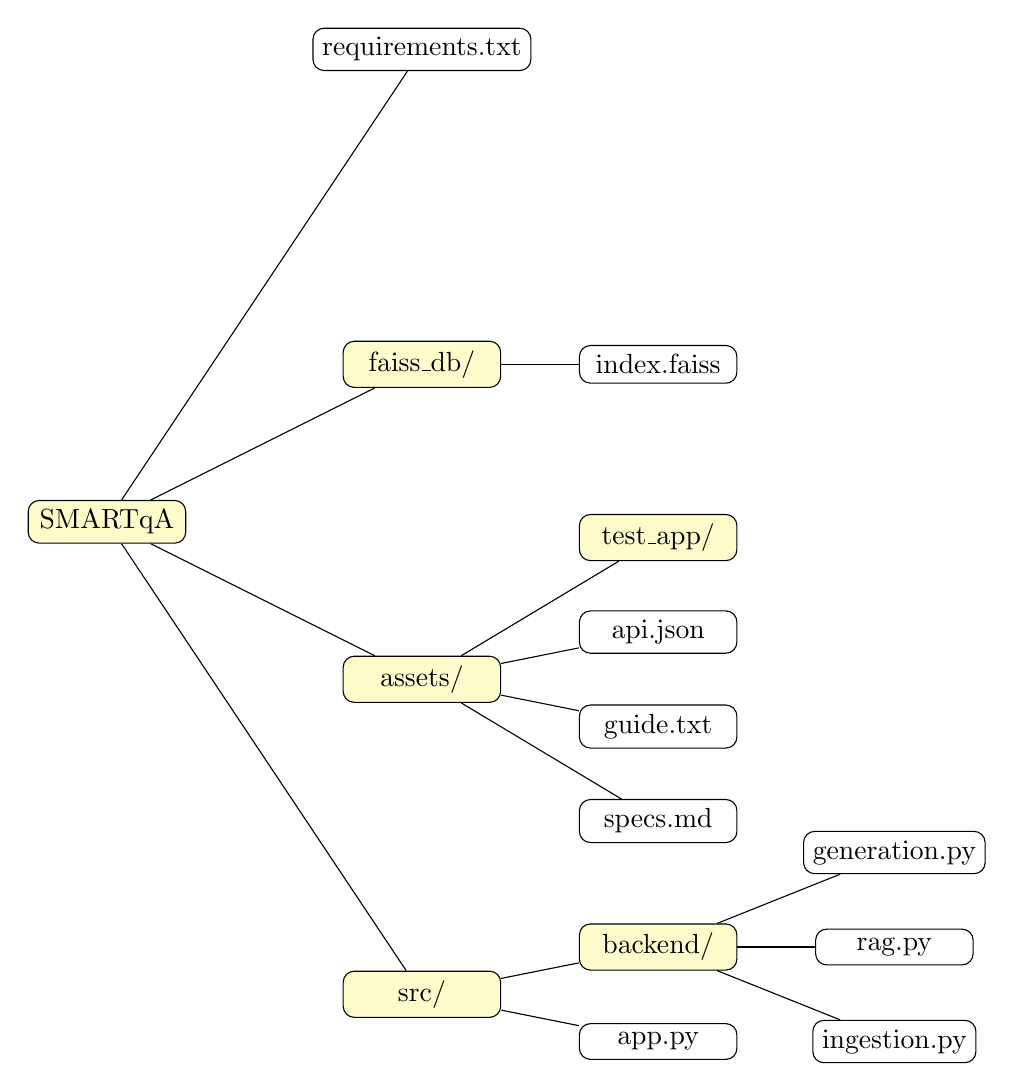
\begin{tikzpicture}[
    grow=right,
    level 1/.style={sibling distance=4cm, level distance=4cm},
    level 2/.style={sibling distance=1.2cm, level distance=3cm},
    folder/.style={draw, fill=yellow!20, rounded corners, minimum width=2cm},
    file/.style={draw, fill=white, rounded corners, minimum width=2cm}
]

\node[folder] {SMARTqA}
    child{node[folder] {src/}
        child{node[file] {app.py}}
        child{node[folder] {backend/}
            child{node[file] {ingestion.py}}
            child{node[file] {rag.py}}
            child{node[file] {generation.py}}
        }
    }
    child{node[folder] {assets/}
        child{node[file] {specs.md}}
        child{node[file] {guide.txt}}
        child{node[file] {api.json}}
        child{node[folder] {test\_app/}}
    }
    child{node[folder] {faiss\_db/}
        child{node[file] {index.faiss}}
    }
    child{node[file] {requirements.txt}};

\end{tikzpicture}
\caption{Project Directory Structure}
\end{figure}

% ============================================
\section{Future Enhancements}
% ============================================

\begin{itemize}
    \item \textbf{Multi-Framework Support}: Playwright and Cypress script generation
    \item \textbf{Multi-Language}: JavaScript, TypeScript, Java test generation
    \item \textbf{Execution Dashboard}: Live test results and reporting
    \item \textbf{CI/CD Integration}: GitHub Actions, Jenkins pipeline support
    \item \textbf{Visual Regression}: Screenshot comparison testing
    \item \textbf{API Testing}: REST and GraphQL test generation
    \item \textbf{Performance Testing}: Load and stress test scenarios
\end{itemize}

% ============================================
\section{Conclusion}
% ============================================

SMARTqA represents a significant advancement in automated testing by combining the power of RAG with modern LLMs to create a truly intelligent QA agent. By grounding all test generation in actual project documentation, it eliminates hallucinations and ensures that tests are always relevant and accurate.

The modular architecture allows for easy extension and customization, while the use of open-source components (FAISS, HuggingFace) ensures cost-effectiveness and local control over sensitive data.

\vspace{1cm}

\begin{tcolorbox}[colback=secondarygreen!10,colframe=secondarygreen,title=Key Takeaways]
\begin{itemize}
    \item \textbf{Zero Hallucination}: All outputs grounded in documentation
    \item \textbf{Production Ready}: Clean, executable Selenium scripts
    \item \textbf{Cost Effective}: Local embeddings, minimal API usage
    \item \textbf{User Friendly}: Intuitive Streamlit interface
    \item \textbf{Extensible}: Modular architecture for easy enhancement
\end{itemize}
\end{tcolorbox}

\end{document}
